\documentclass[a4paper,11pt]{article}
%Premeable
	%Chinese
	\usepackage[UTF8,fontset=fandol]{ctex}
	\usepackage{xeCJK}
	\usepackage[datesep=/]{datetime2}
	\DeclareTextFontCommand{\textbf}{\sffamily}
%Presenting
	\usepackage[table]{xcolor}
	\usepackage{graphicx}
	\usepackage[font={sf}]{caption}
	\usepackage[above]{placeins}
	\usepackage{float,wrapfig}
	\usepackage{tabularx,array,booktabs,multirow,bigstrut}
	\newcolumntype{C}[1]{>{\hsize=#1\hsize%
		\centering\arraybackslash}X}
	\newcommand{\minitab}[2][l]{%
		\begin{tabular}{#1}#2\end{tabular}}
%MathSetting
	\let\latexointop\ointop
	\usepackage{amsmath,bm,amssymb,esint,extarrows}
	\usepackage{upgreek,textcomp,mathrsfs}
	\usepackage[only,sslash]{stmaryrd}
	\usepackage{nicefrac,eqnarray}
%	\usepackage{amsthm}
	\usepackage{mathtools,physics,siunitx}
	\usepackage{stackengine,titling,varwidth}
	\usepackage{tikz}
	\usepackage{resizegather,empheq}
	\usetagform{default}
	\usepackage{calligra,fourier-orns}
	% Keep \oint unchanged by esint
	\let\ointop\undefined
	\let\ointop\latexointop
	% Define a scriptr 
	\DeclareMathAlphabet{\mathcalligra}{T1}{calligra}{m}{n}
	\DeclareFontShape{T1}{calligra}{m}{n}{<->s*[2.2]callig15}{}
	\newcommand{\scriptr}{\mathcalligra{r}\,}
	\newcommand{\rvector}{\pmb{\mathcalligra{r}}\,}
	% Useful shorthand
	\DeclarePairedDelimiter\ave{\langle}{\rangle}
	\newcommand\inlineeqno{\stepcounter{equation}\ (\theequation)}
	\newcommand{\sinc}{\operatorname{sinc}}
	\newcommand{\mbb}[1]{\mathbb{#1}}
	\newcommand{\mrm}[1]{\mathrm{#1}}
	\newcommand{\mcal}[1]{\mathcal{#1}}
	% Scaling and positioning
	\newcommand\scalemath[2]{\scalebox{#1}{\mbox{\ensuremath{\displaystyle #2}}}}
	\newcommand\raisemath[2]{\raisebox{#1\depth}{${#2}$}}
	\empheqset{box=\bbox}
	% Presenting
	\newcommand*\bbox[1]{\fbox{\hspace{1em}\addstackgap[5pt]{#1}\hspace{1em}}}
	\sisetup{%
		redefine-symbols=false,%
		separate-uncertainty=true,%
		range-phrase=\,\textasciitilde\,,%
		arc-separator = \,}
	\allowdisplaybreaks[2]
%ParagraphSetting
	\setlength{\parskip}{.3\baselineskip}
	\usepackage[defaultlines=2,all]{nowidow}
	\postdisplaypenalty=50
%PageSetting
	\usepackage[colorlinks=true,linkcolor=blue]{hyperref}
	\usepackage[vmargin={4cm,5cm},hmargin=3cm,%
		footnotesep=\baselineskip]{geometry}
	\usepackage[bottom]{footmisc}
	\usepackage{changepage}
	% Autoref names
	\renewcommand{\tableautorefname}{\tablename}
	\renewcommand{\figureautorefname}{\figurename}
	% List settings
	\usepackage{enumitem}
	\setlist{itemsep=0pt,topsep=0pt,labelindent=\parindent,leftmargin=0pt,itemindent=*}
	% Some redefined lengths
	\setlength{\headsep}{2.2cm}
	\setlength{\droptitle}{-2.2cm}
	\setlength{\footnotesep}{3\parskip}
	% Header
	\usepackage{fancyhdr,lastpage}
	\pagestyle{fancy}
	\fancyhf{}
	\cfoot{--\ \thepage\,/\,\pageref{LastPage} \ --}
	\renewcommand{\headrulewidth}{0.1pt}
	\renewcommand{\headrule}{
		\vbox to 2pt{
		\hbox to \headwidth{\dotfill}\vss}}
	% Separator
	\newcommand{\newparagraph}{\pagebreak[3]\noindent%
		\hfil
		~\raisebox{-4pt}[10pt][10pt]{\decofourright~~~~~~~~\decofourleft}~ %
		\par
	}
%TitleSettings
	\pretitle{\begin{center}}
	\posttitle{\par\end{center}\vspace{-6mm}}
	\predate{}
	\postdate{\vspace{-4mm}}
%Header
	\lhead{%
		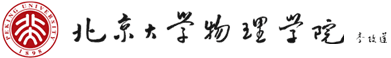
\includegraphics[height=3.2em]{PKUPhy.png}
		\vspace{-3ex}
		}
	\rhead{%
		\itshape\small
		\begin{tabular}{rr}
			\multicolumn{2}{r}{赵启渊} \\[.3em]
			学号:   & 2000011153 \\[.2em]
		\end{tabular}\hspace{-1em}
		}
%Title
	\title{\textit{\large 实验二十三}\\[2mm]
		\textbf{\LARGE 高温超导材料特性测试和低温温度计}}
	\author{\textit{赵启渊} 2000011153}
	\date{}
%Miscellaneous
	\newcommand{\tabindent}{\hspace{2em}}
%FourierTransform
	\newcommand{\ftransform}{\xlongrightarrow{\ \mathscr F\ }}
	\newcommand{\iftransform}{\xlongrightarrow{\ \mathscr F^{-1}\ }}
	\usepackage{gensymb}

\begin{document}
	
	
\maketitle
\thispagestyle{fancy}
\begin{enumerate}
	\item 什么是零电阻效应?零电阻常规导体遵从欧姆定律,它的磁性有什么特点?超导体的磁性又有什么特点?它是否是独立于零电阻性质的超导体的基本特性?\\
	解:材料在常温时是导体或半导体,甚至是绝缘体,当温度下降到某一特定值$ T_c $时,它的直流电阻突然下降为零的效应,称为零电阻效应。\\
	零电阻常规导体,只要$ T < T_c $, 在超导体内部的磁感应强度$B_i$总是等于零,说明具有完全抗磁性。\\
	它是独立于零电阻性质的超导体的另一个基本特性。
	
	
	\item 实验中用到三种低温温度计,分别是什么工作原理? \\
	解:铂电极温度计:在绝对零度下的纯金属中,理想的完全排列的离子实周期场中的电子处于确定状态,电阻为0.温度升高后,由于电子运动状态的改变,会出现电阻。研究表明,当金属纯度很高,且温度在液氮温度以上时,铂电阻温度计的电阻温度关系可以近似表示为$$ R(T) = AT + B $$而且A,B是不随温度变化的常量。用给出的铂电阻温度计在液氮正常沸点和冰点的电阻值,就可以确定A,B,并由此可以测量温度。\\
	通过半导体电阻以及pn结的正向电压测温度: 电子($e^-$)和空穴($e^+$)是半导体导电的粒子,常统称为载流子。在纯半导体中,本征激发产生载流子;在掺杂半导体中,除了本征激发,还有杂质激发。一般来说,在较大温度范围内,半导体具有负的电阻温度系数,适合测量低温。在恒小电流(100$\mu$A)下,近似有$$ U_+ = KT + U_{g0} $$
	$$ K = -2.3 mV/K $$
	q$U_{g0}$是0 K时半导体材料的禁带宽度。\\
	温差电偶温度计: 将两种金属材料制成的导线连成回路,使两个接触点维持在不同的温度,则在该闭合回路中就有温差电动势存在。将一个接触点固定一个已知的温度,则可以由所测量得到的温差电动势确定回路的另一接触点的温度。
	
	\item 测量电路的工作原理是什么?在四引线测量法中,电流引线和电压引线能否互换?为什么?\\
	解:测量电路中电流由恒流源提供,它的大小可以通过标准电阻上的电压测量值得出$$ I = \dfrac{U_n}{R_n} $$
	测得待测样品上的电压,则待测样品上的电阻为$$ R_x = \dfrac{U_x}{I} = \dfrac{U_x * R_n }{U_n} $$
	不能互换,因为如果互换,电流引线与样品的接触点将在电压引线的接触点之间,所测得电压除了待测电阻的,还有电流引线和样品间的接触电阻的,使得测量结果不准。
	\item 如何判断低温恒温器的下档板或紫铜圆筒底部碰到了液氮面?\\
	解:当下挡板碰到液氮面时,除了液面计指示值极剧减小外,还会发出像烧热的铁块碰到水时的响声,同时用手可感到有冷气从有机玻璃板上的小孔喷出。
	\item 确定超导样品的零电阻时,测量电流为何必须反向?这种方法所判定的“零电阻”与实验仪器的灵敏度和精度
	有何关系?\\
	解:超导体电压引线两端的电压值U有$$ U(+) = U_0 + U_1 $$
	$U_0$是乱真电动势引起的,$U_1$是由恒流电流引起的。使电流反向后,$U_1$方向改变,$U_0$没有改变。因此有$$ U(-) = U_0 - U_1 $$
	$$ U_1 = \dfrac{U(+)- U(-)}{2} $$
	因此当$ U(+) = U(-) $时,$ U_1 = 0 $,超导电阻为0.\\
	此时的“零电阻”实际上并不绝对0$\ohm$,而是实验检测到的电阻小于当前的仪器灵敏度。  
	\item 利用硅二极管pn结正向电压随温度变化的线性关系,可以得到那些物理信息?\\
	解:随温度升高,正向电压降低,说明温度越高,硅的禁带宽度越小。 
\end{enumerate}



	\vfill\noindent\itshape\footnotesize
	\hfill Last edited: \today\ \copyright\ 赵启渊
\end{document}